\newpage
\begin{appendix}

%PDF DIN A4 Seiten einbinden: Ort des Dokuments: Hauptordner
\includepdf[frame,pages=1,scale=0.9,pagecommand=\chapter{Auszug aus einem PTB}]{test3}
\includepdf[frame,offset=10mm 5mm,pages=2,scale=0.8,noautoscale=true,pagecommand=\chapter{Noch ein Auszug aus einem PTB}]{test5}


%DIN A3 pdf Seiten einbinden - benötigt noch weitere Anpassungen (Seitenzahl, Ränder, Geometrie)
%\KOMAoptions{paper=A3,paper=landscape, DIV=20}
%\newgeometry{left=4cm, right=2cm, top=2cm}
%\recalctypearea
%\addtokomafont{subsection}{\normalfont\large\rmfamily\mdseries\hspace*{3cm}\vspace{2cm}}
%\includepdf[fitpaper=true,frame,pages=1,scale=0.8,pagecommand=\chapter*{Anhang I: Zeichnung des Dampfablasses}]{test2}


%\KOMAoptions{paper=A4,pagesize, paper=portrait, DIV=20}
%\newgeometry{left=4cm, right=2cm, top=2cm}
%\recalctypearea
% offset=40mm 20mm zum Verschieben der pdf auf der Seite, pagecommand={\thispagestyle{empty}} für Seiten ohne seitenzahl

%delta=8mm 11mm, offset=5mm 7mm,
%trim=0 40mm 0 40mm, clip,  -> 

%Graphiken einfügen
\chapter{Auszug aus der Tabelle xy}
\begin{figure}[ht]
	\centering
  \includegraphics[width=\textwidth]{Anhang/tabelle1.png}
	%\caption{um 30 Grad gedreht}
	%\label{fig1}
\end{figure}





\end{appendix}
